
\section{Plik US-RGB-8-esopecho.dcm}
\begin{frame}
  \frametitle{Plik US-RGB-8-esopecho.dcm}

  \begin{figure}
    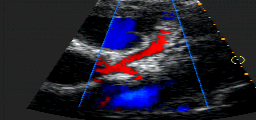
\includegraphics[width=0.4\textwidth]{esopecho}
  \end{figure}
\end{frame}

\begin{frame}
  \frametitle{Informacje ogólne}
  \begin{itemize}
    \item Kodowanie: Explicit
    \item Długość pliku: 93064B, (92160B danych obrazowych, 99\% pliku)
    \item Plik używa grupowania elementów danych
  \end{itemize}
\end{frame}

\begin{frame}
  \frametitle{Dane identyfikujące - \texttt{0x0008}}

  \begin{itemize}
    \item Badanie: Echokardiogram
    \item Data badania (05 listopada 1994 roku, 14:30)
    \item Producent sprzętu (Acme Products)
  \end{itemize}
\end{frame}


\begin{frame}
  \frametitle{Informacje o pacjencie - \texttt{0x0010}}
  Pacjent w tym pliku jest anonimizowany.
\end{frame}

\begin{frame}
  \frametitle{Sposób pozyskania danych obrazowych - \texttt{0x0018}}

  \begin{itemize}
    \item Protokół: Quad Capture
  \end{itemize}
\end{frame}

\begin{frame}
	\frametitle{Informacje o serii - \texttt{0x0020}}
	Jest to obraz numer 107 z 2 serii danych.
\end{frame}

\begin{frame}
  \frametitle{Informacje o obrazie - \texttt{0x0028}}
\begin{itemize}
  \item Każdy piksel składa się z trzech wartości.
  \item Interpolacja RGB
  \item Sposób ułożenia składowych RGB (Planar Configuration)- trzy kolejne warości dotyczą jednego piskela
  \item Rozmiar 120x256
  \item Proporcja pikseli: 4/3
  \item Wartości pikseli są bez znaku
\end{itemize}
\end{frame}

\begin{frame}
  \frametitle{Ukłożenie pikseli w pliku}
  \begin{itemize}
    \item Każdy piksel składa się z trzech wartości: R,G,B, które są ułożone obok siebie.
  \end{itemize}
 $ R_{1,1}, B_{1,1}, G_{1,1}, R_{1,2}, B_{1,2}, G_{1,2}, ..., R_{n,m}, B_{n,m}, G_{n,m} $
\end{frame}
